% !TEX root = ../main.tex

%************************************************
\chapter{Narrow line region properties}
\label{ch:nlr} 
%************************************************

\section{Introduction}

AGN are very efficient at driving outflows; X-ray and UV spectroscopy reveal high velocity outflows to be nearly ubiquituous on sub-parsec scales in high accretion rate quasars.
In recent years, a huge amount of resources have been devoted to searching for observational evidence of galaxy-wide, AGN-driven ouflows, which could provide the feedback mechanism nessecary to quench star formation in massive galaxies. 
This has resulted in recent detections of winds in AGN-host galaxies using tracers of atomic, molecular, and ionised gas \citep[e.g.][]{nesvadba06,arav08,nesvadba08,moe09,dunn10,alexander10,harrison12,harrison14,nesvadba10,rupke13,veilleux13,nardini15,feruglio10,alatalo11,cimatti13,cicone14}.  

One particularly successful technique has been observations of forbiden emission lines, which trace warm (T$\sim10^4$K) ionised gas in the narrow line region (NLR). 
Because of its high equivalent width, [\ion{O}{III}]\l5008 is most studied of the narrow quasar emission lines. 
In general, the [\ion{O}{III}] emission appears to consist of two components: a narrow, `core' component, with a velocity close to the systemic redshift of the host galaxy, and a broader `wing' component, which is normally blueshifted. 
The general consensus is that the core component traces the gravitational potential of the host galaxy, as the width correlates well with the stellar velocity dispersion. 
On the other hand, the wing is tracing outflowing gas. 
This can be explained if the far-side of any outflowing gas, that is moving away from the line of sight, is obscured by dust in the host galaxies \citep[e.g.][]{heckman81,vrtilek85}. 

Observations of broad velocity-widths and asymetries in narrow emission lines stretch back several decades \citep[e.g.][]{weedman70,stockton76,heckman81,veron81,feldman82,heckman84,vrtilek85,whittle85,boroson92}. 
However, the small sample sizes make it difficult to know how representative these observations are. 
More recently, the advent of large optical spectroscopic surveys (e.g. SDSS) have facilitated studies of the NLR in tens of thousands of AGN \citep[e.g.][]{boroson05,greene05a,zhang11,mullaney13,zakamska14,shen14}. 
This has provided constraints on the prevalence of ionised outflows and, by measuring outflow properties as a function of AGN properties, on the drivers of these outflows.  
At the same time, there is strong evidence from spatially resolved spectroscopic observations of kinematically disturbed gas extended over galaxy scales \citep[e.g.][]{greene09,greene11,hainline13,harrison12,harrison14}. 

However, these studies do not cover the redshift range when star formation and black hole accretion peaked, and consequently when feedback is predicted to be strongest. 
At these redshifts the bright optical emission lines are redshifted to near-infrared wavelengths, where observations are much more challenging compared to optical wavelengths. 
As a consequence, studies at high redshifts have typically relied on relatively small numbers of objects, which might not be representative of the properties of the population \citep[e.g.][]{netzer04,sulentic04,shen16a}.
Other recent studies have looked at the [\ion{O}{III}] emission properties of rare sub-samples - e.g. heavily obscured quasars \citep{zakamska16} and the most luminous quasars \citep{bischetti16}. 
These studies often report exceptionally large [\ion{O}{III}] widths, with FWHM $>$ 1000\kms \citep[e.g.][]{netzer04,nesvadba08,kim13,brusa15,carniani15,perna15,bischetti16}. 
This could suggets that AGN efficiency in driving galaxy-wide outflows increases with AGN luminosity. 
In addition, [\ion{O}{III}] is often very weak, or is missing entirely \citep[e.g.][]{netzer04}. 

In this chapter we analyse the [\ion{O}{III}] properties of a sample of 356 high-luminosity, redshift $1.5 < z < 4$ quasars. 
The large sample size will help to put these observations in context of the AGN population as a whole.
We will analyse the [\ion{O}{III}] emission properties as a function of key properties of the quasar, e.g. BH mass, luminosity, and accretion rate. 

\section{Quasar Sample}

We have assembled a catalogue of 356 high-luminosity, redshift $1.5 < z < 4$ quasars.
These are selected from our near-infrared spectroscopic databse (Chapter 2) to have spectra covering the strong, narrow [\ion{O}{III}] doublet. 
The broad Balmer \hb line is also observed for all but two of the sample. 
In 165 the spectra extend to the broad \ha emission at 6565\AA, and in 260 optical spectra including \ion{C}{IV} are also available (mostly from SDSS/BOSS). 
This is the largest study of the narrow line region properties of high-$z$ quasars ever undertaken. 
The quasar sample is summarised in Table~\ref{tab:specnums_ch4}.

\begin{table}
  \centering
  \small 
  \caption{The numbers of quasars with [\ion{O}{III}] line measurements and the spectrographs and telescopes used to obtain the near-infrared spectra.}
  \label{tab:specnums_ch4}
    \begin{tabular}{ccc} 
    \hline
    Spectrograph & Telescope & Number \\
                 &           & \\
    \hline
    FIRE         & MAGELLAN  & 31 \\
    GNIRS        & GEMINI-N  & 28 \\
    ISAAC        & VLT       & 9 \\
    LIRIS        & WHT       & 7 \\
    NIRI         & GEMINI-N  & 29 \\
    NIRSPEC      & Keck II   & 3 \\
    SINFONI      & VLT       & 80 \\
    SOFI         & NTT       & 76 \\
    TRIPLESPEC   & ARC-3.5m  & 27 \\
    TRIPLESPEC   & P200      & 45 \\
    XSHOOTER     & VLT       & 21 \\
    \hline
    & & 356 \\
    \hline
    \end{tabular}
\end{table} 

\section{Parameteric Model Fits}

In this section we describe how parameters of the [\ion{O}{III}] emission are derived. 
Our approach is to first model the spectra, and then derive parameters of interest from the best-fitting model. 
This enhances the useful information that can be extracted from spectra with finite signal-to-noise (S/N). 

Two different models are considered.
The first consists of a power-law continuum, an empirical \ion{Fe}{II} template and multiple Gaussian components to model the emission from the broad and narrow components of \hb and the [\ion{O}{III}] doublet. 
This is a model which is commonly adopted in the literature \citep[e.g.][]{shen11}. 
The second model consists of six spectral components derived from an independent component analysis (ICA) of a large sample of low-redshift AGN with SDSS spectra covering the same spectral region.
As we will demonstrate, a linear combination of these spectral components is able to reproduce the spectra around \hbns/[\ion{O}{III}] to a high degree of precision.  

\subsection{Model One: Multiple Gaussians}

The first step in our procedure is to fit a combination of a power-law continuum and an optical \ion{Fe}{II} template -- taken from \citet{boroson92} -- to two windows at 4435-4700 and 5100-5535\,\AA.
The \ion{Fe}{II} template is convolved with a Gaussian, and the width of this Gaussian, along with the normalisation and velocity offset of the \ion{Fe}{II} template, are free variables in the pseudo-continuum fit.

This requires the spectra to be transformed to within $\sim$1000\kms\, of the quasar rest-frame. 
The redshift used in this transformation is either derived from the peak of the broad \ha emission ($\sim$ 40 per cent of our sample), from the peak of the broad \hb emission ($\sim$ 40 per cent) or from the peak of the narrow [\ion{O}{III}] emission (20 per cent).
In later sections, emission line locations will always be quoted as relative velocities, and so do not explicitly depend on how the quasar rest-frame is defined at this stage in the fitting procedure.  

Once the continuum and \ion{Fe}{II} emission has been modelled and removed, the following model is fit in the wavelength interval 4700-5100\,\AA.
The fit is done as a function of the Doppler velocity shift, and we adopt the wavelength 4862.721\AA\, (the laboratory \hb wavelength) to transform wavelengths into equivalent Doppler velocities.

In general, \hb is modelled by two Gaussians with non-negative amplitudes and FWHM greater than 1200\kms.
In 10 objects \hb is modelled with a single Gaussian and in 41 objects \hb is modelled with two Gaussians, but the velocity centroids of the two Gaussians are constrained to be equal. 
These spectra generally have low signal-to-noise (S/N), and adding extra freedom to the model does not significantly decrease the minimised reduced chi-squared.
In addition there are cases where the blue wing is below the lower wavelength limit of the spectrograph; in these cases models with more freedom are insufficiently constrained by the data with limited wavelength converage. 

Contributions to the \hb emission from the narrow-line region is weak in the vast majority of our sample, and in general we do not include an additional Gaussian component to model this emission. 
In 9 objects features in the model - data residuals suggest that a narrow emission component is significant, and an additional narrow Gaussian is included for these quasars. 
It is likely that there is some not insignificant contribution from the narrow line region in other quasars. 
If this is the case then measures of the \hb velocity width will be biased to lower values on average. 
However, in this chapter we are only interested in location of the peak of the \hb emission (to infer the quasar redshift). 
This is unlikely to be biased by not decomposing the narrow and broad emission components. 

Each component of the [\ion{O}{III}] doublet is fit with one or two Gaussians, depending on the fractional reduced $\chi^2$ difference between the one- and two-component models. 
If the addition of the second Gaussian decreases the reduced $\chi^2$ by more than 5 per cent then the double-Gaussian model is accepted.
One hundred and thirty-one are fit with a single Gaussian and 154 with two Gaussians. 
When a single Gaussian is used to model each line, the peak flux ratio of the [\ion{O}{III}] 4960\,\AA\, and 5008\AA\, components are fixed at the expected 1:3 ratio and the width and velocity offsets are set to be equal.
In the double Gaussian fit, the peak flux ratio of the second components is again fixed at 1:3, and the width and velocity offsets are again set to be equal. 

In 71 objects [\ion{O}{III}] is undetected, or is very low S/N. 
In these cases we do not attempt to measure the width of the [\ion{O}{III}] emission, but instead fit a fixed [\ion{O}{III}] template, only the overal normalisation of which is allowed to vary. 
The template is derived by running our fitting routine on a very high S/N composite spectra of low redshift AGN. 
\todo{Composite details?}

Model parameters were derived using a standard variance-weighted least-squares minimisation procedure employing the Levenberg-Marquardt algorithm. 
Prior to the fit, the spectra were inspected visually and regions significantly affected by telluric absorption or of low S/N were masked out.
Some example fits are shown in Figure~\ref{fig:example_spectrum_grid}

\begin{figure*}
    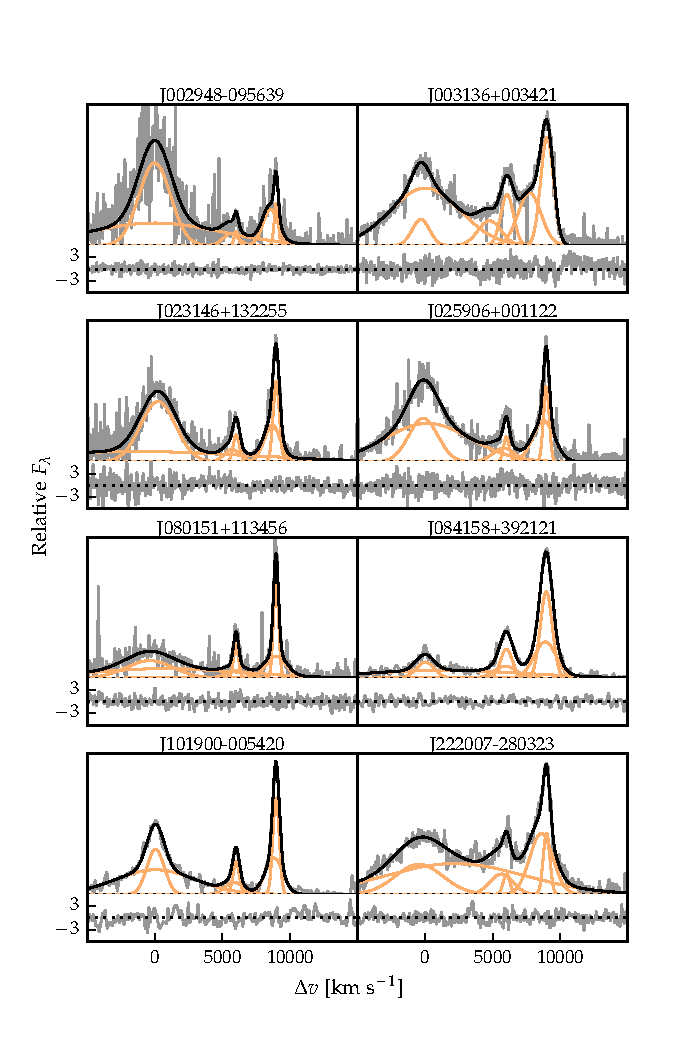
\includegraphics[width=\textwidth]{figures/chapter04/example_spectrum_grid.pdf} 
    \caption{Multi-component Gaussian fits to the continuum-subtracted \hbns/[\ion{O}{III}] emission in 12 quasars, chosen to be the representative of the wide range of [\ion{O}{III}] line widths we measure in our sample. The data is shown in grey, the best-fitting parametric model in black, and the individual model components in orange. Below each fit we plot the data minus model residuals, scaled by the errors on the fluxes.}     
    \label{fig:example_spectrum_grid}
\end{figure*}


\subsection{Derived parameters}

All [\ion{O}{III}] line properties are derived from the [\ion{O}{III}]5008 emission, but, as described above, the kinematics of the peak at 4960\AA\, are constrained by our fitting routine to be identical.

We do not to attach any physical meaning to the individual Gaussian components used in the model. 
While it is true that in some quasars the [\ion{O}{III}] emission can be clearly separated in to a narrow component at the systemic redshift and a lower-amplitude, blueshifted broad component \citep[e.g.][]{shen16a}, often this decomposition is highly uncertain and dependent on the spectral S/N, resolution etc.
In addition, there is no theoretical justification that wing component should have a Gaussian profile.  

We therefore choose to characterize the [\ion{O}{III}] line profile using a number of non-parameteric measures, which are commonly used in the literature \citep[e.g.][]{zakamska14,zakamska16}. 
A normalised cumulative velocity distibution is constructed from the best-fitting model, from which the velocities below which 5, 10, 25, 50, 75, 90, and 95 per cent of the total flux accumulates can be read off. 
The width of the emission line can then be defined, for example, using $w_{80} = v_{90} - v_{10}$. 
The absolute assymetry in the line profile $A$ is defined as $((v_{95} - v_{50}) - (v_{50} - v_{5})) / (v_{95} - v_{5})$ \citep{zakamska14}. 
We use the peak of the full [\ion{O}{III}] profile to define the systemic redshift, and verify below that this is unbiased.  
\todo{The line width measures are not corrected for instrumental broadening}
\todo{Add outline of table of derived properties for this chapter}

\subsection{Absolute flux calibration of spectra and continuum luminosities}

Relative flux-calibration of the infrared spectra as a function of wavelength has been achieved, to $\simeq$10 per cent, through observations of appropriate flux standards. 
The absolute flux levels, however, can be in error by large factors due to variable atmospheric conditions combined with the narrow slit widths. 
For the majority of the quasars we have, therefore, established the absolute flux scale for each near-infrared spectrum using the same quasar SED-model fitting scheme employed in Chapter~\ref{ch:sed}.
Briefly, the SED-model was fit, with the normalisation and E(B-V) as free varibales, to optical/infrared magnitudes, or SDSS/BOSS spectra (check order I do this.)
This allows us to extrapolate from the optical when we do not have photometric data in the near-infrared. 
The spectra were then normalised to the SED model using a linear error-weighted least-squares regression in the the regions of the spectra covered by the $H$/$K$ bands. 
The monochromatic continuum luminosity at 5100\AA was calculated directly from the normalised SED-model. 
\todo{Check if any missing normalisation / monochromatic luminosities.} 
\todo{I think a lot of this is repeated from chapter 2/3}
\todo{Check factor of (1+z) in luminosity calculation}

\subsection{Reliability of derived parameters}

\subsubsection{Removal of \ion{Fe}{II} emission}

\begin{figure}
    \centering
    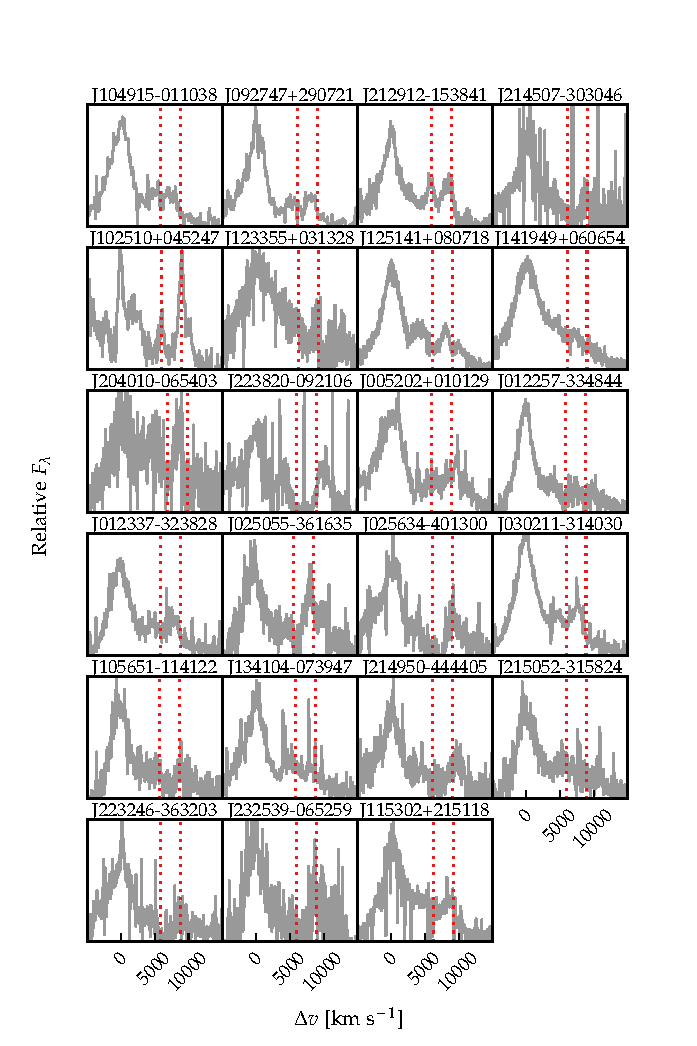
\includegraphics[width=\columnwidth]{figures/chapter04/example_spectrum_grid_extreme_fe.pdf} 
    \caption{The continuum and \ion{Fe}{II} spectra of the 23 objects we identified where the \citet{boroson92} empirical template is a poor match to the \ion{Fe}{II} emission. The vertical lines indicate the expected positions of the [\ion{O}{III}] doublet (which is generally very weak) with a systemic redshift defined using the peak of the broad \hb emission.}     
    \label{fig:bad_fe}
\end{figure}

While we were able to satisfactorily model the \ion{Fe}{II} emission in the vast majority of cases, we encountered a number of cases where the relative strengths of the \ion{Fe}{II} lines appear to differ significantly from those of I Zw 1 on which the \ion{Fe}{II} template is based. 
As a result, significant \ion{Fe}{II} flux remained in the spectrum after the removal process. 
This emission is at rest-frame wavlengths very close to the [\ion{O}{III}] emission, and so could potentially lead to large errors in the inferred [\ion{O}{III}] line parameters. 

In Figure~\ref{fig:bad_fe} we plot the spectral region around [\ion{O}{III}] for 23 quasars we have identified where significant features remain following the subtraction of the continuum and \ion{Fe}{II}. 
The vertical lines indicate the expected positions of the [\ion{O}{III}] doublet, with zero velocity defined using the peak of the broad \hb emission. 
[\ion{O}{III}] is generally exteremely weak in these objects. 
As a result, the widely-adopted procedure of fitting multiple Gaussians will tend to fit the \ion{Fe}{II} emission as broad, shifted [\ion{O}{III}]. 
For example, J125141+080718 was studied by \citet{shen16a}, and assigned an extremely large [\ion{O}{III}] blueshift. 
Our analysis suggets that this emission is more likely to be \ion{Fe}{II}. 
Because of the difficulty measuring the [\ion{O}{III}] properties of these objects, they are excluded from subsequent analysis.  

\subsubsection{Low EQW [\ion{O}{III}]}

\begin{figure}
    \centering
    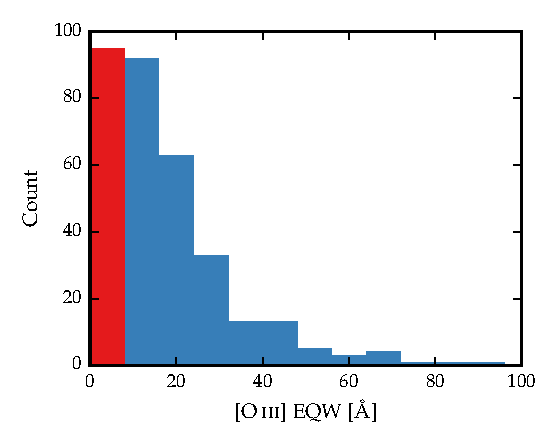
\includegraphics[width=0.6\textwidth]{figures/chapter04/oiii_eqw_hist.pdf} 
    \caption{[\ion{O}{III}] Rest-frame equivalent width of 330 quasars in our sample. The [\ion{O}{III}] profiles of the 120 objects in the red bin (EQW $<$ 8\AA) cannot be measured reliably, and so these objects are excluded from our analysis.}     
    \label{fig:oiii_strength_hist}
\end{figure}

In Figure~\ref{fig:oiii_strength_hist} we show the distribution of the [\ion{O}{III}] rest-frame EQW distribution for the 330 objects in our sample (objects where \ion{Fe}{II} emission has been sub-optimally removed are excluded). 
In many objects [\ion{O}{III}] is undetected. 
In others it is detected, but is too weak for its shape (i.e. the width and asymmetry) to be measured reliably. 
We define EQW$=8$\AA as the limit below which we can no longer reliably determine the shape of the [\ion{O}{III}] emission. 
Objects with EQW$<8$\AA (120) are excluded in subsequent analysis of the [\ion{O}{III}] shape.  

\subsubsection{Low S/N [\ion{O}{III}]}
 
\begin{figure}
    \centering
    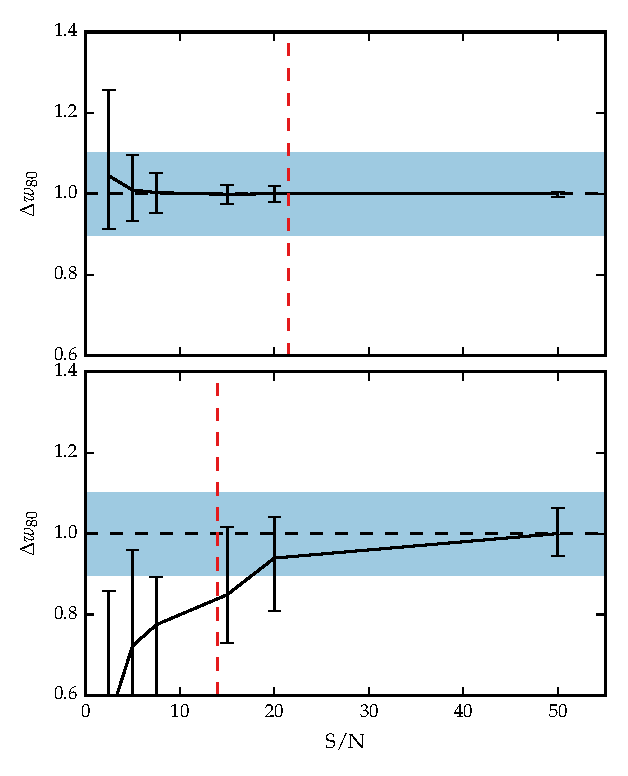
\includegraphics[width=0.7\columnwidth]{figures/chapter04/snr_test.pdf} 
    \caption{}
    \label{fig:snr_test}
\end{figure}

In this section we flag objects with poor spectral S/N. 
A single S/N cut is not adequate: for a given S/N, it is much easier to measure the properties of a strong line than a weaker one. 
Our approach is therefore as follow:

\begin{enumerate}
\item For each object use the best-fitting parametric model as a high S/N representation of the spectra. 
\item Scale the error spectrum so that the S/N (measured in the continuum and quoted per pixel) is \{2.5, 5, 7.5, 10, 15, 20, 50\}.
\item At each S/N, generate 100 mock spectra by randomly drawing the flux in each pixel from a Normal distribution with mean $\mu$ equal to the model flux and width $\sigma$ equal to the scaled error. 
\item Run line-fitting procedure on each mock of the 100 mock spectra; record the value of $w_{80}$ in the best-fitting model. 
\item Calculate the 16th, 50th and 84th percentiles of the distribution of $w_{80}$ values.
\item A low S/N flag is assigned to the object if the value of $w_{80}$ changes by more than 10 per cent from the highest S/N representation to the S/N of the data. 
\end{enumerate}

Two examples are shown in Figure~\ref{fig:snr_test}.
The marker denotes the 50th percentile, and the lower and upper error bars the 16th and 84th percentiles respectively. 
As expected, the uncertainty on $w_{80}$ increases as the S/N of the spectrum decreases. 
The S/N in to two spectra are similar, but the [\ion{O}{III}] line in the  first object is stronger. 
Hence it can still be measured reliably even at low S/N. 
The first object would pass our S/N cut, whereas the latter would fail. 

\subsection{Model Two: Independent Component Analysis}

Independent component analysis (ICA) is a blind source separatation tecnique for separating a signal in to linearly mixed statistically independent subcomponents. 
Unlike the more widely-used principle component analysis technique, ICA produces non-negative components which allows for a physical interpretation of the components and weights.  
ICA has been succesfully applied to model the spectra of emission-line galaxies \citep{allen13} and BAL quasars \citep{allen11}. 
The quasar spectra can be thought of as a set of observations, $\bm{x}$, which are made up of statistically independent components, $\bm{c}$, that are combined by some mixing matric, $\bm{W}$:

\begin{equation}
    \bm{x} = \bm{W}\bm{c}
\end{equation}

ICA reverses this process and describes how the observed data are generated. 
Both the independent components and the mixing matrix are unknown, but can be found by solving:

\begin{equation}
    \bm{c} = \bm{W}^{-1}\bm{x}.
\end{equation}

The components were solved for using a sample of 2,154 SDSS quasars at redshifts XX. 
\todo{Ask Paul for details.}
At these redshifts the SDSS spectrograph covers the rest-frame region XX-XX\AA\, where \hb and [\ion{O}{III}] lie. 
The individual spectra were first adjusted to give the same overall shape as a model quasar template spectrum.
Six positive independent components and four additional components that could be negative were found to be sufficient to reconstruct the spectrum, without over-fitting. 
Each quasar spectrum can then be represented as a linear combination of the independent components: 

\begin{equation}
    x_j = \sum_{i=1}^{10} c_{ij}W_{ij}
\end{equation}

\subsubsection{Fitting procedure}

For each quasar in our NIR sample we perform a variance-weighted least-squares minimisation to determine the optimum value of the components weights.
The fitting procedure we employ is as follows. 
A power-law is first fit to the quasar template spectrum in emission line free windows at 4200-4230, 4435-4700 and 5100-5535 \AA. 
Each of the ICA components is then divided by the power-law. 
An identical process is performed on each of the spectrum to be fitted, so that there is essentially zero shape in both the components and the spectrum to be fitted. 
The first six component weights are constrained to be non-negative, and the fit is done in logarithmic wavelength space, so that each pixel corresponds to a fixed velocity width.   

\subsubsection{Quality of fits}

In general, the ICA components do a remarkably good job at reconstructing the spectra of the objects in our sample. 
For example, in J125141+080718 (discussed above), it does much better job at modelling the \ion{Fe}{II} emission than the \citet{boroson92} template. 
It is less sensitive to the spectral S/N, and the component weights do not need to be constrained. 
It is therefore much simpler to apply than fitting multiple Gaussians. 

However, it does have its limitations. 
The components were calculated using a set of lower-redshift, lower-luminosity AGN, and quasar spectra are known to vary systematically as a function of luminosity. 
For example, the [\ion{O}{III}] line is typically broader in more luminous quasars. 
Because there are so few objects with very broad [\ion{O}{III}] in the low-redshift sample, the ICA reconstuction fails to reproduce the broadest [\ion{O}{III}] profiles in our sample. 

\subsection{Physical interpretation of ICA components}

\begin{figure}
    \centering
    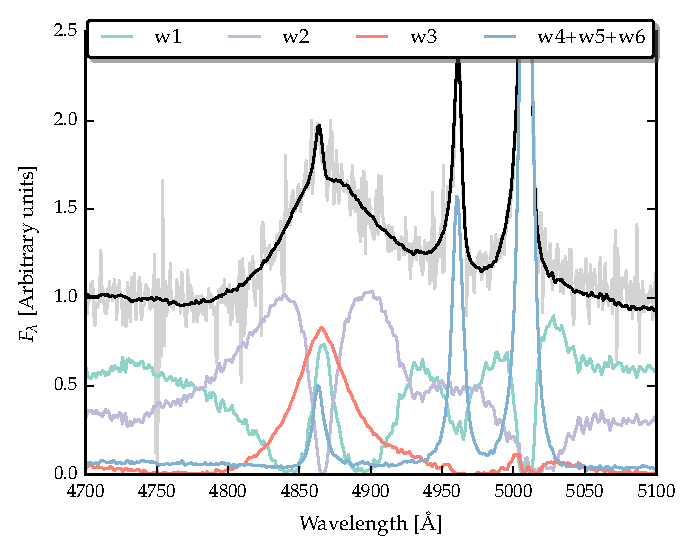
\includegraphics[width=0.8\textwidth]{figures/chapter04/mfica_components.pdf} 
    \caption{ICA reconstruction of spectrum. The total profile is shown in black, and the six individual positive components are shown with different colours. The component weights are the median values from our fits to the low- and high-luminosit samples.}     
    \label{fig:mfica_components}
\end{figure}

Although the ICA is analysis is not based on any physics,  there appears to be a direct correspondence between the individual components and the different emission features which contribute to the spectra (Fig.~\ref{fig:mfica_components}). 
This correspondence is summarised in Table~\ref{tab:icacomps}. 
The component $w_1$ seems to correspond to \ion{Fe}{II} emission, the components $w_2$ and $w_3$ to broad \hb emission, the components $w_4$ and $w_5$ to narrow [\ion{O}{III}] emission at the systemic redshift, and the component $w_6$ to broad, blueshifted [\ion{O}{III}] emission. 

\begin{table}
  \centering
  \caption{Approximate physical origin of the ICA components.}
  \label{tab:icacomps}
    \begin{tabular}{cc} 
    \hline
    Component & Origin \\
    \hline
    $w_1$& \ion{Fe}{II} \\
    $w_2$& \hbns \\
    $w_3$& \hbns \\
    $w_4$& [\ion{O}{III}] core \\
    $w_5$& [\ion{O}{III}] core \\
    $w_6$& [\ion{O}{III}] wing \\
    \hline
    \end{tabular}
\end{table} 

\subsubsection{Reconstructing the [\ion{O}{III}] profile}

\begin{figure}
    \centering
    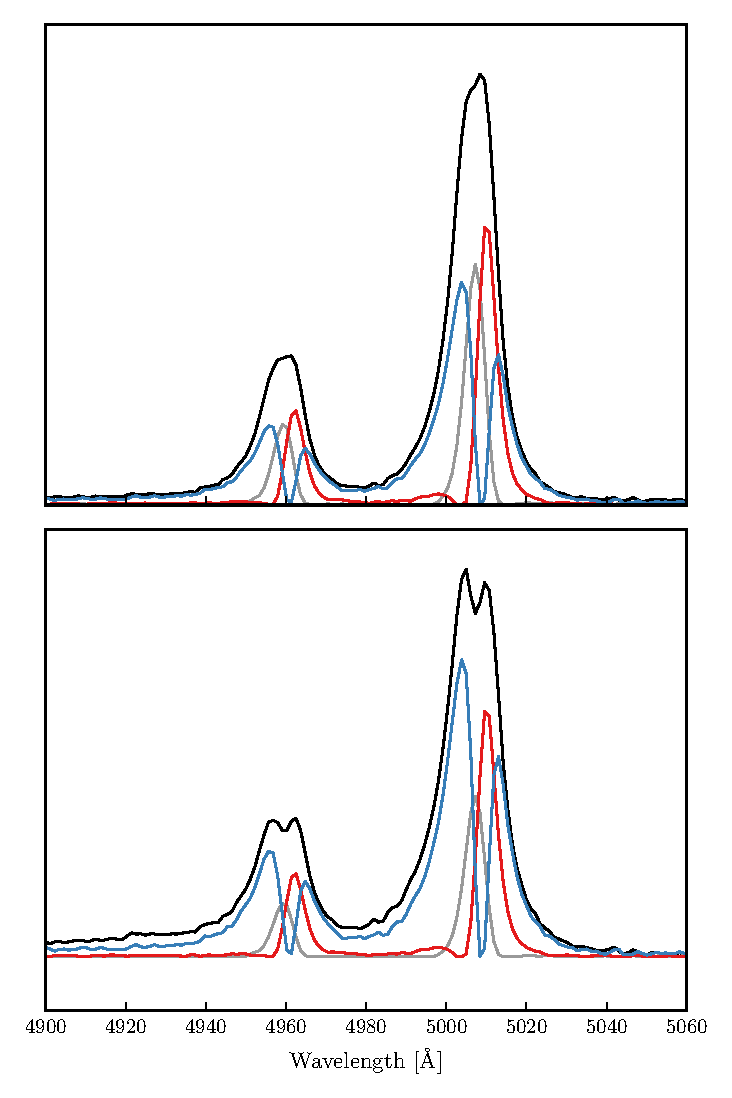
\includegraphics[width=0.8\columnwidth]{figures/chapter04/mfica_components_oiii_comparison.pdf} 
    \caption{Comparison of median [\ion{O}{III}] profiles from ICA fits it low- and high-luminosity samples. }     
    \label{fig:mfica_components_oiii_comparison}
\end{figure}

In order to measure non-paramteric line parameters, e.g. $v_10$, we must first reconstruct the [\ion{O}{III}] emission. 
It is fortunate that most of the [\ion{O}{III}] emission is in just three of the ICA components; the remaining three contribute very little. 
Therefore, we can set the first three weights to zero to leave only the [\ion{O}{III}] emission. 

We define the boundaries of [\ion{O}{III}]\l5008 as being between 4950 and 5500\AA. 
The blue limit is close to the peak of the [\ion{O}{III}]\l4960 line, and so to recover the intrinsic profile we instead use the blue wing of [\ion{O}{III}]\l4960. 
We use the emission from 4980-5050\AA, and from 4900-(4980-(5008.2-4960.3)). 
The blue window is then shifted by (5008.2-4960.3) to reconstruct the blue wing of the [\ion{O}{III}]\l5008 line. 

The reconstructed spectra are shown in Figure~\ref{fig:mfica_components_oiii_comparison}. 
At present I am summing the flux all the way from 4950\AA. 
However, this is quite a lot of flux to sum up, and we can't ascribe this flux to the wing of the [\ion{O}{III}] emission with any certainty. 
This is bourne out by the fact that there are quite large differences between, for example, $v_{10}$ measured from the Gaussian fit and $v_{10}$ measured from the ICA fit. 

\section{Results}

\subsection{Gaussian fits}

\begin{figure}
    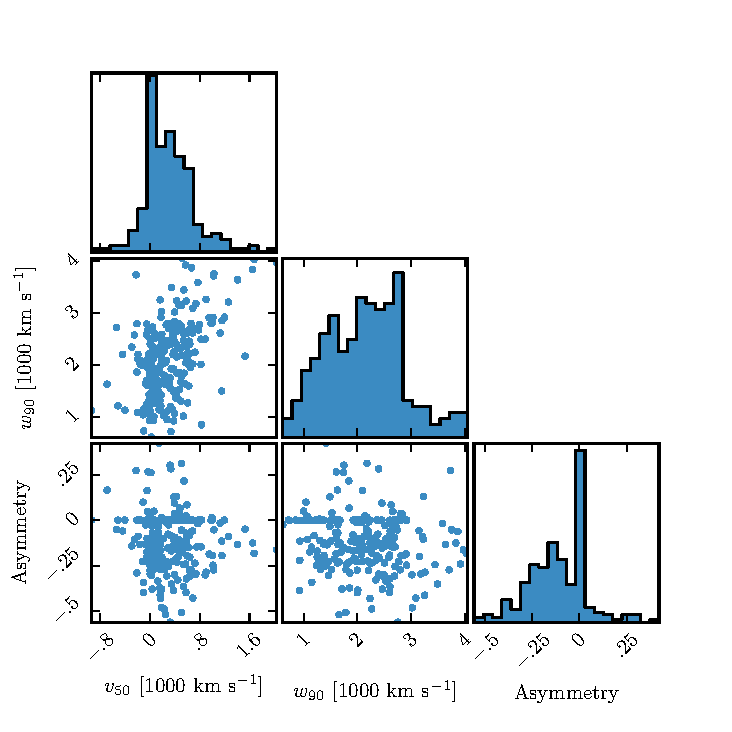
\includegraphics[width=\columnwidth]{figures/chapter04/parameters_grid.pdf} 
    \caption{The distributions of and correlations between a subset of the non-parameteric measures we made of the best-fitting [\ion{O}{III}] models. \todoinline{Remake adding EQW and blueshift? Expain reason for zero asymmetry (single Gaussian)}}     
    \label{fig:parameters_grid}
\end{figure}

Our best-fitting profiles show a strongly blue-asymmetric profile (Fig.~\ref{fig:parameters_grid}), with a significant fraction of the total emission in a blue wing.
The luminous blueshifted broad wing and the exteremely broad profile reveals high-velocity outflowing ionized gas. 
Our results, and those of other authors, suggest that kpc-scale outflows in ionized gas are common among the most luminous high-redshift actively accreting SMBHs.

We see a correlation between the [\ion{O}{III}] velocity width and blueshift. 
As the blueshift of the line increases it gets broader. 
This is consistent with \citet{shen14}, where the strength of the narrow core is decreasing, leading to a broader and more blueshifted profile. 

\subsubsection{Eigenvector 1 correlations}

At low redshifts, it is standard to use principle component analysis (PCA) to define quasar extrema. 
This has led to the so-called EV1 correlates \citep{boroson92}. 
Specifically, much of the variance in quasar spectra is reflected in an anti-correlation between the relative strength of \ion{Fe}{II} and the \hb FWHM. 
These emission line trends in the optical (for low-$z$ quasars) can be extrended to UV emission lines observed at higher redshifts. 
The \ion{C}{IV} blueshift and EQW is a diagnostic that similarly spans the diversity of broad emission line properties in high redshift quasars (dominated by a virialized component at one extreme and a wind driven component at the other) \citep{richards11,sulentic07}. 
The similarity of the \ion{C}{IV} EQW-blueshift parameter space at high redshift to EV1 parameter space at low redshift suggetss that these trends are connected. 

Can we calculate a mapping between the two parameter spaces? 
As a first step we show how the EV1 parameters change as a function of position in the \ion{C}{IV} EQW-blueshift parameter space in Figure~\ref{fig:ev1}. 
Most of the diversity in \ion{C}{IV} properties seems to be driven by the [\ion{O}{III}] EQW. 
On the other hand, properties of the \ion{C}{IV} line cannot be used to predict the \hb FWHM. 
This is similar to what we found in Chapter~\ref{ch:bhmass}: objects with large \ion{C}{IV} blueshifts have narrow Balmer emission lines, but objects with modest \ion{C}{IV} blueshifts have a wide range of Balmer line widths. 

Can do something similar with ICA weights, but I'm not sure what the best question to ask is. 
Could make a linear model of the ICA component weights and fit to the \ion{C}{IV} blueshift? 

\begin{figure}
    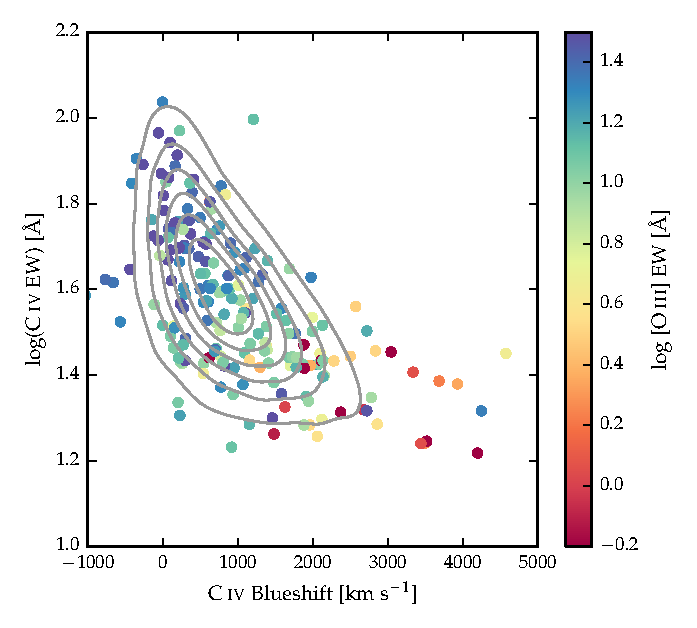
\includegraphics[width=\columnwidth]{figures/chapter04/ev1.pdf} 
    \caption{The [\ion{O}{III}] EQW as a function of the \hb FWHM and the optical \ion{Fe}{II} strength (EQW \ion{Fe}{II}/ EQW \hb).}     
    \label{fig:ev1}
\end{figure}

\subsubsection{Extreme [\ion{O}{III}]}

\begin{figure}
    \centering
    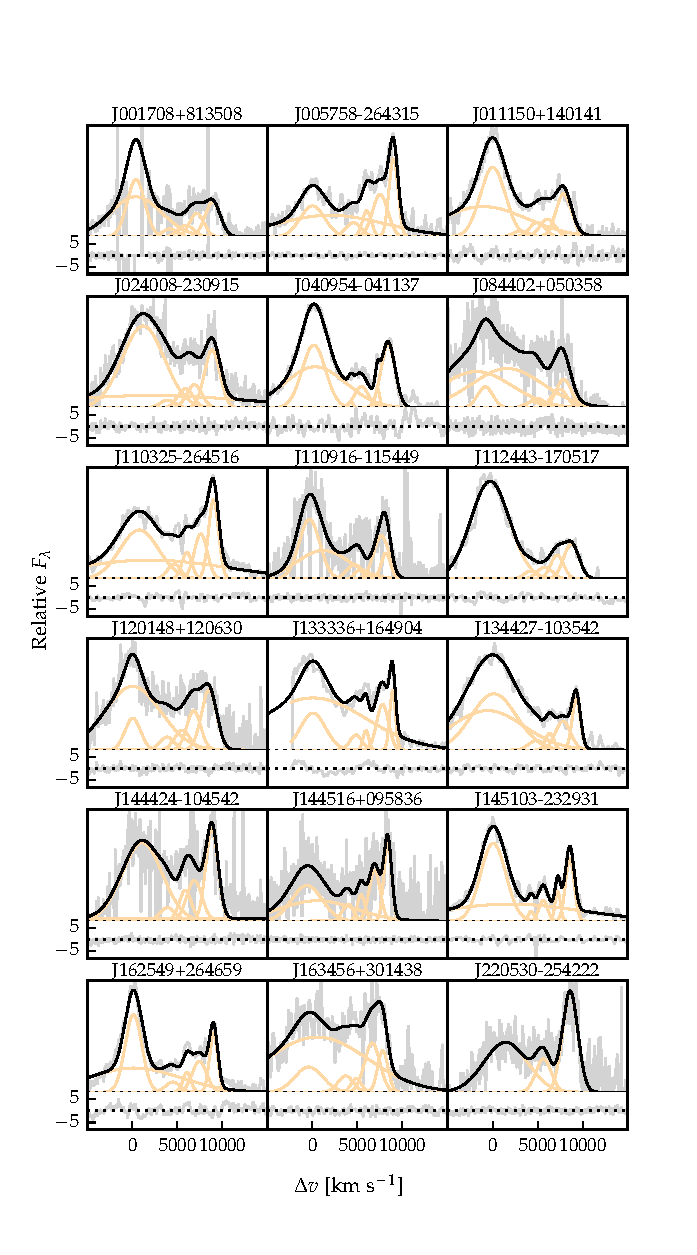
\includegraphics[width=1\columnwidth]{figures/chapter04/example_spectrum_grid_extreme_oiii.pdf} 
    \caption{Extreme [\ion{O}{III}] emission profiles.}     
    \label{fig:example_spectrum_grid_extreme_oiii}
\end{figure}


Because of this diversity, it is the dominant variable in the set of correlations making up EV1, which is believed to be linked to certain fundamental parameters of the accretion process. 
In Figure~\ref{fig:ev1} we show the [\ion{O}{III}] EQW as a function of the \hb FWHM and the optical \ion{Fe}{II} strength. 
The optical \ion{Fe}{II} strength is defined as the ratio of the \ion{Fe}{II} and \hb EQW, where the \ion{Fe}{II} EQW is measured between 4434 and 4684\AA.
These parameters form part of `eigenvector 1' (EV1), the first eigenvector in a principal component analysis which originated from the work of \citet{boroson92}.
In our sample, these parameters follow very similar correlations to what is observed at low-$z$ \citep[e.g.][]{shen14}.
In particular, the anti-correlation between the [\ion{O}{III}] and \ion{Fe}{II} EQWs.  

Same as \citet{shen16a}, we confirm that the EV1 correlations hold at high luminosities/redshifts. 
See also Sulentic et al. 2004, 2006; Runnoe et al. 2013. 
Make sure it's clear that \citet{shen16a} quasars make up a significant chunk of our sample. 

\subsection{ICA fits}

\begin{figure*}
    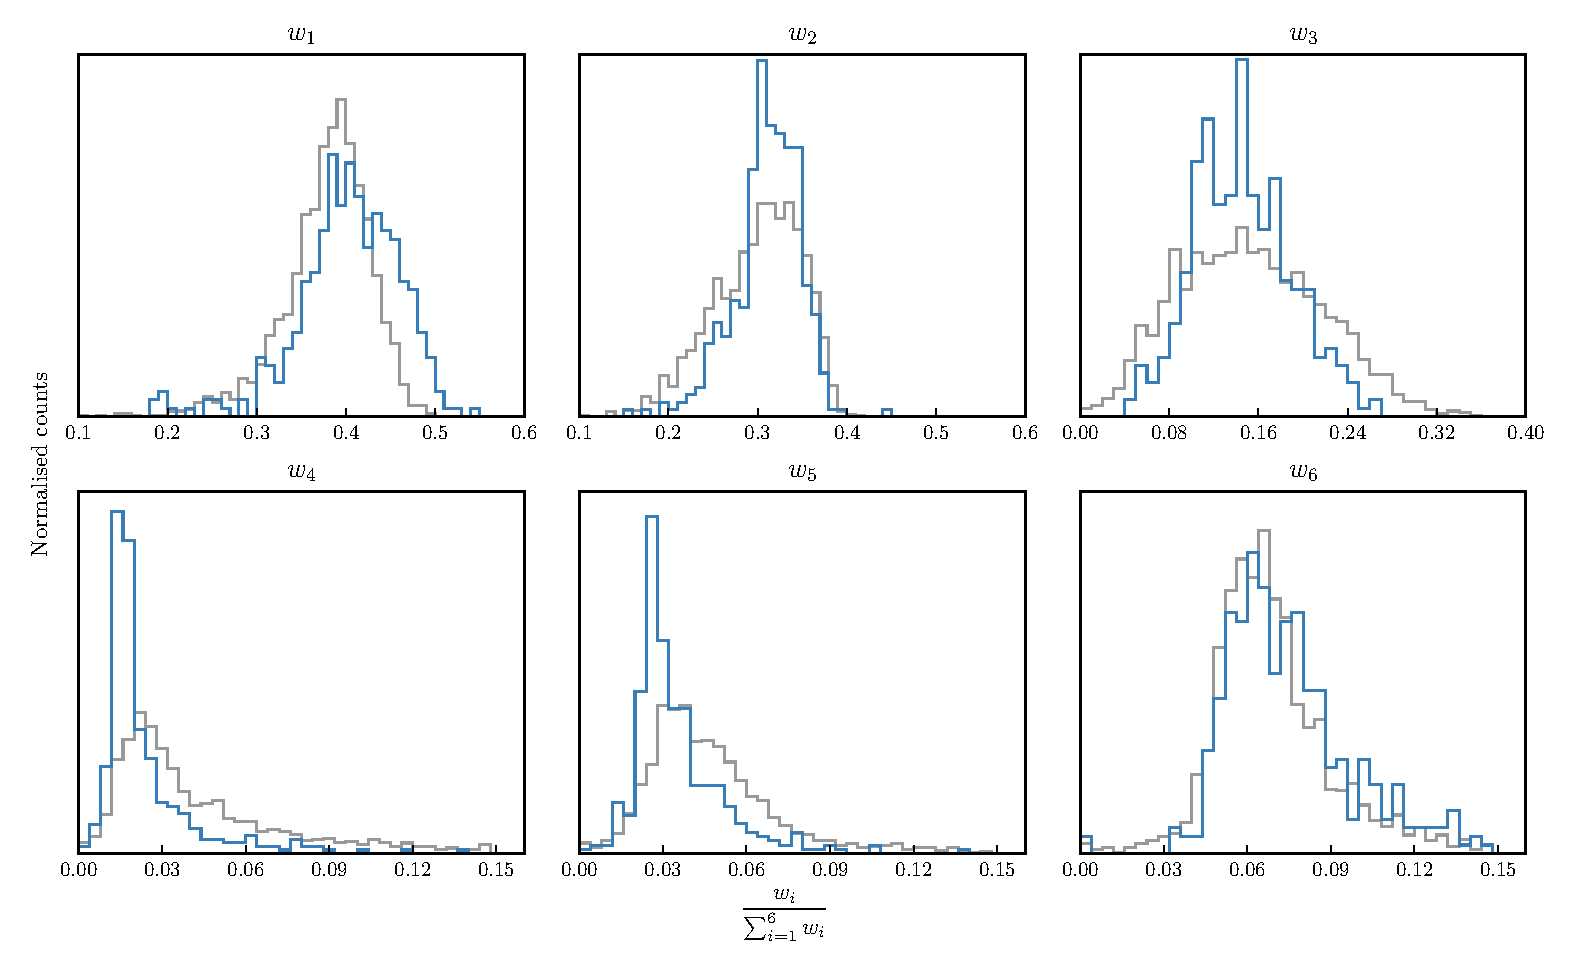
\includegraphics[width=\textwidth]{figures/chapter04/mfica_component_weights.pdf} 
    \caption{The relative weight in each of the six positive ICA components for the high-luminosity (blue) and low luminosity samples (grey). In the high-luminosity sample \ion{Fe}{II} emission is stronger (component $w_1$). The core [\ion{O}{III}] emission is weaker (components $w_4$, $w_5$) but the strength of the blueshifted wing is the same ($w_6$).}     
    \label{fig:mfica_component_weights}
\end{figure*}

\begin{figure*}
    \centering
    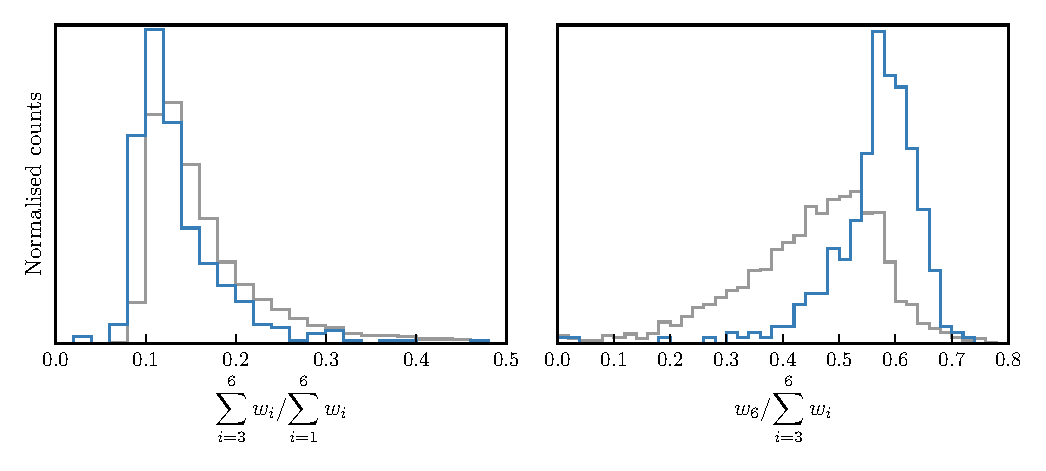
\includegraphics[width=\textwidth]{figures/chapter04/mfica_oiii_weight.pdf} 
    \caption{The relative weight in the three ICA components corresponding to [\ion{O}{III}] emission ({\em left}) and the relative weight of the component most closely related to blueshifted [\ion{O}{III}] emission relative to all three [\ion{O}{III}] components ({\em right}). [\ion{O}{III}] emission is weaker in the high-luminosity sample, but the relative contribution but the fractional contribution from the blueshifted component to the total [\ion{O}{III}] emission is higher. Hence [\ion{O}{III}] is weaker, broader, and more asymmetric in the high-luminosity sample.}     
    \label{fig:mfica_oiii_weight}
\end{figure*}

\begin{figure}
    \centering
    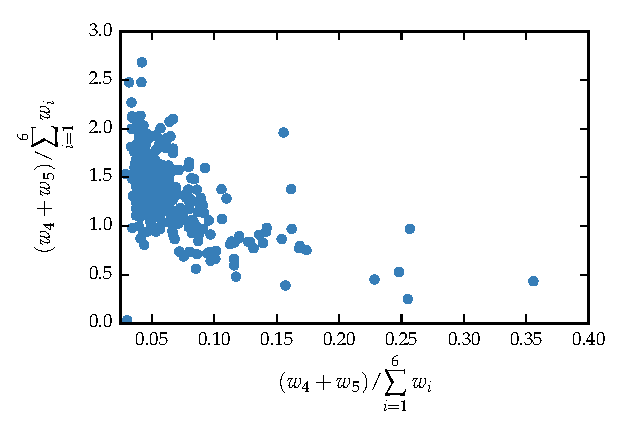
\includegraphics[width=\columnwidth]{figures/chapter04/oiii_core_strength_blueshift.pdf} 
    \caption{}     
    \label{fig:oiii_core_strength_blueshift}
\end{figure}

We find there is a decreasing symmetric component at high luminosities. 
Relates directly to \citet{shen14}. 
A stable narrow line region is removed by the outflowing material. 
\citet{shen14} showed that the strength of the core [\ion{O}{III}] component decreases with quasar luminosity and optical \ion{Fe}{II} strength faster than the wing component, leading to overall broader and more blueshifted profiles as luminosity and \ion{Fe}{II} strength (or \ion{C}{IV} blueshift) increases. 

Zhang et al. 2011: Blueshift of [\ion{O}{III}] correlates significantly with the EQW of the core. 
The more the peak of the line is blueshifted, the more the core component decreases dramatically, while the blue wing changes much less. 
We see this clearly in Figure~\ref{fig:oiii_core_strength_blueshift}. 
This is similar to behaviour of \ion{C}{IV}? i.e. is there a mapping from this to the \ion{C}{IV} space diagram? This would suggests that the mechamism producing the two corerlations is the same. 
Consistent with the core coming from the canonical extended NLR where the gas is dominate by gravity of the bulge while the wing arises in an outflow. 
And \ion{C}{IV} explained by wind. Suggests intimate connection between BLR and NLR.

\subsubsection{EV1 correlations}

\begin{figure}
    \centering
    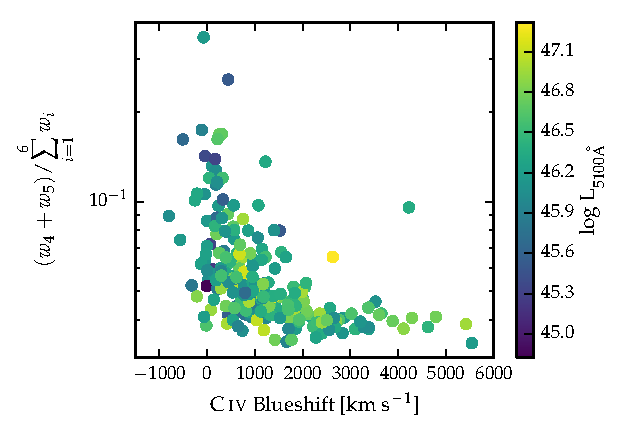
\includegraphics[width=\textwidth]{figures/chapter04/civ_blueshift_oiii_strength.pdf} 
    \caption{[\ion{O}{III}] strength decreases as the \ion{C}{IV} blueshift increases. See similar thing if I use [\ion{O}{III}] EQW instead. Only showing the core components here. The \ion{C}{IV} blueshift is now measured relative to the NIR ICA redshift. I think this is trend is mostly being driven by the Eigenvector 1 correlations: as the blueshift increases the \ion{Fe}{II} strength increases and the [\ion{O}{III}] strength decreases. Doesn't appear to be driven by the luminositiy. Is this tighter than EV1 trend shown with Fe/OIII strength by other authors? Is the AGN NLR absent in objects where outflows have reached
    kiloparsec scales, sweeping up the low-density material responsible for the [OIII]-emission?}     
    \label{fig:civ_blueshift_oiii_strength}
\end{figure}

\begin{figure}
    \centering
    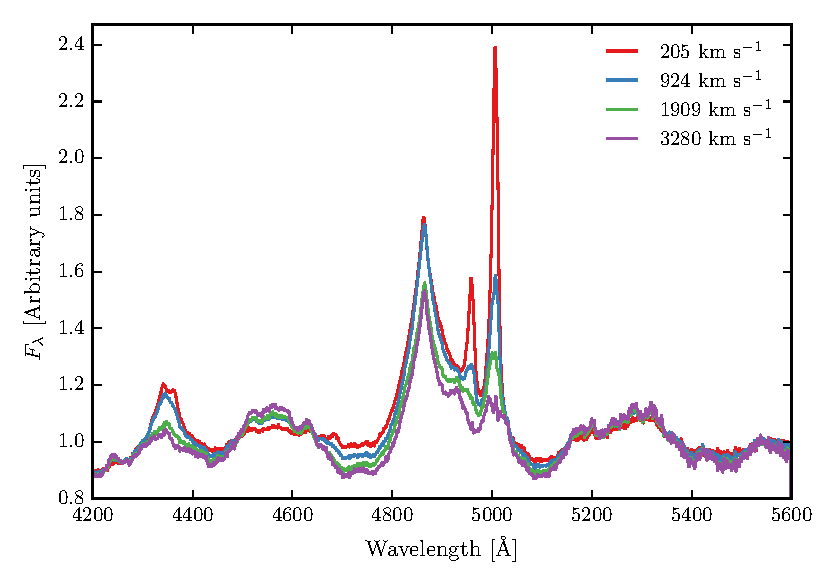
\includegraphics[width=\columnwidth]{figures/chapter04/mfica_composites.pdf} 
    \caption{ICA median weights as a functino of the CIV blueshift.}     
    \label{fig:mfica_composites}
\end{figure}

In Figure~\ref{fig:civ_blueshift_oiii_strength} we show how the [\ion{O}{III}] strength varies as a function of the \ion{C}{IV} blueshift. 
There is a very well defined relation: when \ion{C}{IV} is strongly blueshifted [\ion{O}{III}] is very weak. 

This is shown in a different way in Figure~\ref{fig:mfica_composites}. 
Here we divide our sample in to four bins according to the \ion{C}{IV} blueshift. 
From the quasars in each \ion{C}{IV} blueshift bin we then find then generate an ICA spectrum using the median weights from each quasar. 
The differences in the spectra as a function of the \ion{C}{IV} blueshift are dramatic. 
[\ion{O}{III}] becomes progressively weaker and more blueshifted.
The anti-correlation with \ion{Fe}{III} and the blueward \ion{Fe}{II} also clear, but there is no change in the redward \ion{Fe}{II}. 

This seems to really connect high-z EV1 with low-z EV1, which I don't think has really been done before. 
At low redshifts we have the strengths of [\ion{O}{III}], \ion{Fe}{II}, and the \hb FWHM. 
At high redshifts we have the \ion{C}{IV} blueshift and EQW. 
The distribution of quasars in these two planes look qualitatively similar.  
It's tempting to think that quasars with large \ion{C}{IV} blueshifts should also have strong \ion{Fe}{II} and weak [\ion{O}{III}]. 
This is indeed what our results seem to suggets. 

The ICA can be thought of as update on EV1. 
The spectral diversity is encapsulated in the EV1 components. 
Most of the variance in EV1 is the anti-correlation between the strengths of [\ion{O}{III}] and \ion{Fe}{II}. 
So at one end we have objects with strong \ion{Fe}{II} and weak [\ion{O}{III}], and at the other end objects with weak \ion{Fe}{II} and strong [\ion{O}{III}]. 
Other properties, including the \ion{C}{IV} blueshift and the \hb FWHM, also change systematically. 
Our work shows that the ICA component weights change systematically along the EV1 sequence. 
\todo{What is the best way to actually do this mapping?}. 

\section{Measuring the quasar systemic redshift}

\begin{figure}
    \centering
    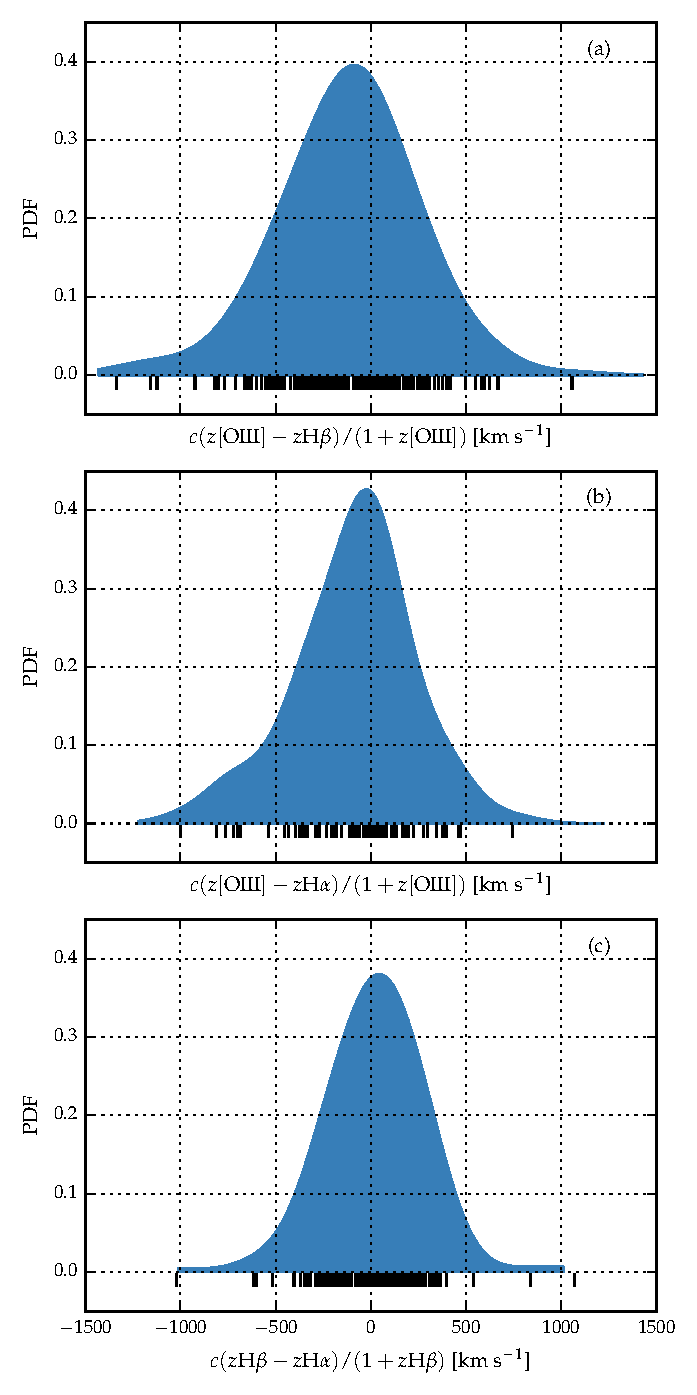
\includegraphics[width=0.8\linewidth]{figures/chapter04/redshift_comparison.pdf} 
    \caption{Redshift comparisons. Lots have been excluded from Ha/Hb so need to look at flags greater than one. What is the big peak? Gaussian fit to the first one has failed. Find out why these plots look different to ones in paper.}       
    \label{fig:redshift_comparison}
\end{figure}

In this section we do a comparison of systemic redshift estimates from [\ion{O}{III}], broad \hb and \hans, and from fitting the ICA component weights. 
This is an important issue. 
Accurate systemic redshift estimates are essential in a number of applications, and researchers have devoted a large amount of telescope time to obtaining near-infrared spectra to access [\ion{O}{III}] for this purpose. 
HI, CO and absorption line mesaures of the host galaxy rest frame suggest that [\ion{O}{III}] usually gives consistent results within 200 km/s (de Robertis 1985; Whittle 1985; Wilson \& Heckman 1985; Condon et al. 1985; Stripe 1990; Alloin et al. 1992; Evans et al. 2001).  
However, our work shows that at high luminosities this can result in large errors (profile can be dominated by blueshifted component, Fe emission can be improperly subtracted, or [\ion{O}{III}] might not be detected at all. 

\subsection{\hans}

There are 224 quasars in our sample with spectra covering the \ha emission line. 
We discard seven of these from our sample because of very low S/N ($<$2.5 measured in the \ha line), leaving 217
To measure the position of the line we fit a parameteric model, which is very similar to the model described in Chapter~\ref{ch:bhmass}. 
The continuum emission is first modeled and subtracted using the procedure described in Chapter~\ref{ch:bhmass}. 
We then test five different models with increasing degrees of freedom to model the \ha emission. 
The models are summarised in Table~\ref{tab:hamod}. 
They are (1) a single broad Gaussian; (2) two broad Gaussians with identical velocity centroids; (3) two broad Gaussians with different velocity centroids; (4) two broad Gaussians with identical velocity centroids, and additional narrower Gaussians to model the narrow \ha emission, and the narrow components of [\ion{N}{II}]\ll6548,6584 and [\ion{S}{II}]\ll6717,6731; (5) two broad Gaussians with different velocity centroids, and additional narrower Gaussians. 
If used, the width and velocity of all narrow components are set to be equal in the fit, and the relative flux ratio of the two [\ion{N}{II}] components is fixed at the expected value of 2.96.
The model we select is the simplest model for which the fractional change in the reduced chi-squared from the model with the lowest reduced chi-squared is less than ten per cent. 
The redshift is then measured at the peak flux of the \ha model, including both the broad and narrow components of \ha if appropriate. 

\begin{table}
  \centering
  \small 
  \caption{Models used for \ha emission}
  \label{tab:hamod}
    \begin{tabular}{cccc} 
    \hline
    Model     & Components & Fix centroids? & Number \\
    \hline
    1        & 1 broad Gaussian  & N/A &  10 \\
    2        & 2 broad Gaussians & Yes &  71 \\
    3        & 2 broad Gaussians & No  &  32 \\
    4        & 2 broad Gaussians + narrow Gaussians & Yes & 51 \\
    5        & 2 broad Gaussians + narrow Gaussians & No  & 53 \\
    \hline
    \end{tabular}
\end{table} 

\subsection{ICA}

\todo{Need to recalculat ICA redshifts since shift to fit in log space}. 
Benefit of ICA is that it works regarless of the [\ion{O}{III}] strength. 

Can also describe what I found trying to get redshifts from broad \hans, \hbns? (Narrow components generally very weak at these luminosities so can't be used.)
Generally find no systematic errors but large ($\sim$1000\kms\, scatter).
Comparing NIR ICA to [\ion{O}{III}] for the [\ion{O}{III}] with high S/N I find small (few hundred \kms) scatter. 



















\section{Luminosity/redshift-evolution of [\ion{O}{III}] properties}

\begin{figure}
    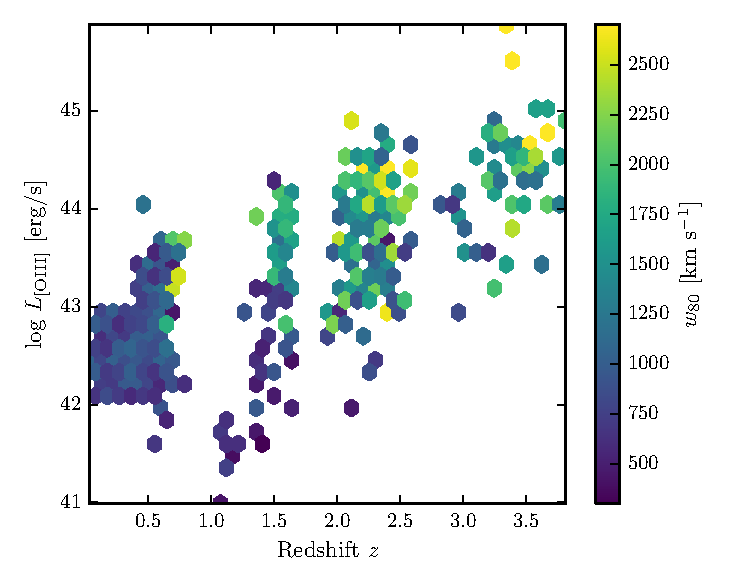
\includegraphics[width=\columnwidth]{figures/chapter04/oiii_luminosity_z_w80.pdf} 
    \caption{The [\ion{O}{III}] velocity-width, characterised by $w_{80}$, as a function the [\ion{O}{III}] luminosity and the quasar redshift. The color of each hexagon denotes the mean $w_{80}$ for the obects in that luminosity-redshift bin. We have suplemented our sample with low-$z$ objects from \citet{zakamska14} and medium ($z\sim$1.5) redshift objects from \citet{harrison16}. If I keep this plot make sure its clear which points belong to which sample.}       
    \label{fig:oiii_luminosity_z_w80}
\end{figure}

In this section we look for any luminosity/redshift dependent changes in the [\ion{O}{III}] line properties. 
To do this we extend the dynamic range of our samples in terms of both luminosity and redshift by supplementing our sample with quasars presented by \citet{zakamska14} and \citet{harrison16}. 

The \citet{zakamska14} objects are a sample of 568 obscured luminous quasars selected from SDSS \citep{reyes08,yuan16}. 
They are selected to have [\ion{O}{III}] luminosities above $10^{8.5}{\rm L}\odot$ and have a median redshift $z=0.397$. 

We also include 40 quasars at redshifts $1.1 \leq z \leq 1.7$) from the KMOS AGN Survey at High redshift (KASH$z$) with [\ion{O}{III}] line measurements. 

We also have the same information for $\sim$20\,000 SDSS spectra from \citet{mullaney13}. 

In Figure~\ref{fig:oiii_luminosity_z_w80} we show the [\ion{O}{III}] velocity width as a function of the [\ion{O}{III}] luminosity and the quasar redshift. 
The lack of any redshift-evolution between $z=0$ and $z=1.5$ was reported by \citet{harrison16}.
Our additional data suggets that this continues to $z\sim2.5$. 
On the other hand, at fixed redshift, we see a significant correlation between the [\ion{O}{III}] velocity width and the luminosity. 

The fact that we don't see many broad lines in the \citet{zakamska14} objects even at luminosities $>$43 erg/s could be due to the fact that these are all type II quasars, whereas the sample presented in this chapter are all type I. 
\citet{mullaney13} showed that the [\ion{O}{III}] lines of type I quasars are typically broader than in type II quasars. 

\section{Equivalent width}

\begin{figure}
    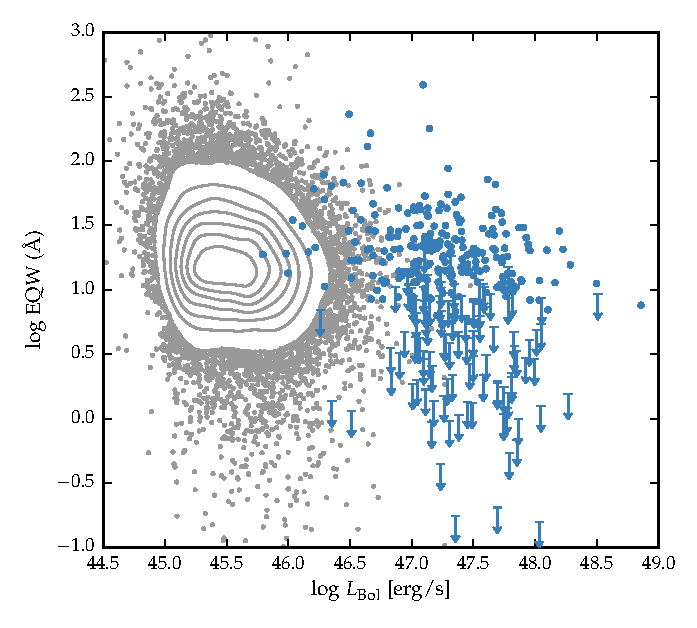
\includegraphics[width=\columnwidth]{figures/chapter04/eqw_lum.pdf} 
    \caption{The [\ion{O}{III}] EW as a function of the quasar bolometric luminosity for the sample presented in this chapter (blue circles) and the low-$z$ SDSS sample (grey points and contours). Upper limits are denoted by the downward arrows.}     
    \label{fig:eqw_lum}
\end{figure}

Firstly, the best-fitting model comprising the continuum, \ion{Fe}{II}, and \hb emission is subtracted from the spectra, leaving behind only emission due to [\ion{O}{III}]. 
From this spectra we generate 100 mock spectra, where the flux at each wavelength is randomly drawn from a Normal distribution with a mean equal to the flux convolved with a Gaussian of width 200\kms and a width equal to the known error. 
We then perform an error-weighted linear least-squares regression with an [\ion{O}{III}] template derived from a fit to a very high S/N low redshift SDSS composite spectra. 
The equivalent width of the best-fitting model is recorded for each of the 100 realisations of the spectra. 
The error in the equivalent width is defined as the root-mean-square of these values.

In Fig.~\ref{fig:eqw_lum} we show the [\ion{O}{III}]5008 EW as a function of the quasar bolometric luminosity. 
Bolometric luminosity is estimated from the monochromatic continuum luminosity at 5100\AA using the correction factor given by \citet{richards06}. 
For comparison, we also show the low-$z$ sample from \citet{shen11}.  

The equivalent width of [\ion{O}{III}] has been found to strongly decrease as a function of redshift and/or luminosity \citep[e.g.][]{brotherton96,netzer04,sulentic04,baskin05b}. 

The size of the narrow line region is roughly expected to scale as $L^{0.5}$ \citep[e.g.][]{netzer04}. 
However, for high luminosity quasars with strong [\ion{O}{III}] this gives NLR sizes which are unreasonably large \citep[$\sim$100 kpc;][]{netzer04}. 

\citet{netzer04} found 1/3 of their high luminosity sample had very weak [\ion{O}{III}], whereas quasars with weak [\ion{O}{III}] are very rare for nearby AGN. 
We find that [\ion{O}{III}] is undetected/very weak in XX per cent of our sample, which is very similar to the fraction reported by \citet{netzer04}.  
\citet{netzer04} claim that for the population of strong [\ion{O}{III}] emitters there is no reduction of EW with increasing source luminosity. 
On the other hand, there are many weak or no [\ion{O}{III}] emitters at high luminosity that could give the impression that the line EQW decreases with increasing source luminoisity. 


\subsection{[\ion{O}{III}] and \ion{C}{IV} outflows are linked}

\begin{figure}
    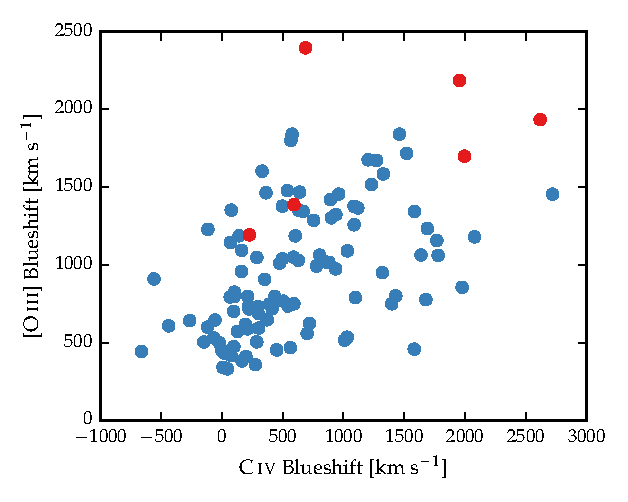
\includegraphics[width=\columnwidth]{figures/chapter04/civ_blueshift_oiii_blueshift.pdf} 
    \caption{The relation between the blueshifts of \ion{C}{IV} and [\ion{O}{III}]. Note that we are using $v_{10}$ for the [\ion{O}{III}] position and $v_{50}$ for the \ion{C}{IV} position. We can't use $v_{50}$ for [\ion{O}{III}] because sometimes we are using a single Gaussian, especially if the [\ion{O}{III}] is weaker and we miss the broad component.}     
    \label{fig:oiii_civ_blueshifts}
\end{figure}

Optical spectra are available for XXX quasars in our catalogue, and cover the broad \ion{C}{IV} doublet. 
As we described in Chapter~\ref{ch:bhmass}, \ion{C}{IV} is often blueshifted, which almost certainly signal the presence of strong outflows, most likely originating in a disc wind.
In Chapter~\ref{ch:bhmass} we demonstrated that the quasars in our sample cover the full range of \ion{C}{IV} blueshifts seen in the SDSS quasar population, which makes our sample unique in that it allows us to study properties of the quasar across the full parameter range. 

The \ion{C}{IV} velocity centroid measurements are taken directly from Chapter~\ref{ch:bhmass}. 
We define the `location' of the [\ion{O}{III}] emission using $v_{10}$, although the results are the same if $v_{20}$, $v_{50}$ etc. are used instead.

In Figure~\ref{fig:oiii_civ_blueshifts} we show the \ion{C}{IV} blueshifts against the [\ion{O}{III}] blueshifts.
This comparison is done for a sub-sample of 146 objects where we have good measurements of the \ion{C}{IV}, [\ion{O}{III}] profiles. 

There is a clear and strong correlation. 
Note that our EQW cut removes most of the quasars with large \ion{C}{IV} blueshifts, since [\ion{O}{III}] is on average very weak in these qusars. 
Similar correlations have been tentatively found in lower redshift quasars and AGN \citep{zamanov02}. 

The blueshifting of \ion{C}{IV} is known to correlate with luminosity \citep{richards11}.
In [\ion{O}{III}], the blueshifted wing becomes relatively more prominent as the luminosity of the quasar increases \citep{shen14}. 
Therefore, it is plausible that the correlation between the \ion{C}{IV} and [\ion{O}{III}] blueshifts is a secondary effect that is driven by the correlation of each with the luminosity. 
However, no strong luminosity-dependent trends are apparent in Figure~\ref{fig:oiii_civ_blueshifts}. 
We find that both the [\ion{O}{III}] and \ion{C}{IV} blueshifts are correlated with the luminosity, but that these correlations are much weaker than the correlation between the [\ion{O}{III}] and \ion{C}{IV} blueshifts. 



\section{Eigenvector one correlations}



\section{Broad Absorption Line Quasars}

\todo{Check all of this}
19 quasars in our catalogue are classified as broad absorption line (BAL) quasars, using the either the SDSS classification flags or the \citet{allen11} catalogue. 
We find that the BAL quasars have typically broader [\ion{O}{III}] than the rest of the sample. 
Note that in the \citet{zakamska16} sample of very red quasars, the incidence of BALs is very high, and these objects have extremely broad [\ion{O}{III}] profiles. 
A two-sided Kolmogorov-Smirnov statistic on the $w_{80}$ distributions returned a p-value of 0.10. 
What does this mean?
Try with different parameters?
Histograms look rubbish so maybe just give the numbers. 

\section{Discussion}

Looking at the [\ion{O}{III}] velocity width as a function of luminosity tells us about the physical drivers of the outflows observed in [\ion{O}{III}]. 
The correlation with luminosity suggests that the highest velocity outflows are associated with the most luminous AGN. 
This has been reported for low-redshift AGN, for both ionized and molecular outflows (e.g. Westmoquette et al. 2012; Veilleux et al. 2013; Arribas et al. 2014; Cicone et al. 2014; Hill \& Zakamska 2014).

This suggests that the outflows are driven by radiative forces. 
On the other hand, \citet{mullaney13} find that once the correlation between the [\ion{O}{III}] luminosity and the radio luminosity has been taken in to account, the [\ion{O}{III}] velocity width is more strongly related to the radio luminosity of the AGN. 

\subsection{Type II quasars}

Implications of our findings on searches for high-redshift type 2 quasars. It could be that type II quasars exist. If you look at CIV/MgII the narrow line components are very weak. So the contribution from the narrow line region is very weak in luminous quasars, and you just won't see it even if the broad line region is obscured.
Findings in this paper seem to suggest that the startic narrow line region is very weak in luminous quasars. 


